\documentclass[11pt,a4paper]{report}
\usepackage[T1]{fontenc}
\usepackage[utf8]{inputenc}
\usepackage[english]{babel}
\usepackage{lmodern}
\usepackage{geometry}
\geometry{margin=25mm}
\usepackage{amsmath,amssymb,booktabs,array,longtable,xcolor,graphicx,hyperref,fancyhdr,tikz,listings,float}
\usetikzlibrary{arrows.meta,positioning,shapes.geometric}
\hypersetup{colorlinks=true,linkcolor=blue!50!black,urlcolor=blue!50!black}
\definecolor{navy}{HTML}{15324F}
\definecolor{pale}{HTML}{EDF3F8}
\definecolor{codegreen}{HTML}{226644}
\newcommand{\hex}[1]{\texttt{#1}}
\newcommand{\xor}{\mathbin{\oplus}}
\newcommand{\rol}{\mathbin{\lll}}
\newcommand{\note}[1]{\par\smallskip\noindent\colorbox{pale}{\parbox{0.94\linewidth}{\textbf{Note.} #1}}\par\smallskip}
\pagestyle{fancy}\fancyhf{}\fancyhead[L]{\small AES and SM4: Fault Analysis}\fancyhead[R]{\small PFE 5A}\fancyfoot[C]{\thepage}
\setlength{\headheight}{14pt}
\lstdefinestyle{pycode}{language=Python,basicstyle=\ttfamily\scriptsize,keywordstyle=\color{blue!55!black},commentstyle=\color{codegreen},breaklines=true,breakatwhitespace=true,frame=single,backgroundcolor=\color{pale},numbers=left,numberstyle=\tiny\color{gray},xleftmargin=7mm,columns=fullflexible,showstringspaces=false}
\lstdefinestyle{terminal}{basicstyle=\ttfamily\scriptsize,breaklines=true,frame=single,backgroundcolor=\color{black!4},columns=fullflexible,showstringspaces=false}
\lstset{style=pycode}
\begin{document}
\begin{titlepage}
\centering
\vspace*{8mm}
\begin{minipage}{.45\linewidth}\centering
\IfFileExists{polytech_montpellier_logo.png}{
\includegraphics[width=.9\linewidth,height=24mm,keepaspectratio]{polytech_montpellier_logo.png}}{\fbox{\parbox[c][23mm][c]{.9\linewidth}{\centering\bfseries Polytech Montpellier\\\small Upload logo PNG}}}
\end{minipage}\hfill
\begin{minipage}{.45\linewidth}\centering
\IfFileExists{stmicroelectronics_logo.png}{
\includegraphics[width=.9\linewidth,height=24mm,keepaspectratio]{stmicroelectronics_logo.png}}{\fbox{\parbox[c][23mm][c]{.9\linewidth}{\centering\bfseries STMicroelectronics\\\small Upload logo PNG}}}
\end{minipage}
\vspace{30mm}
{\color{navy}\rule{\linewidth}{1.5pt}}\par\vspace{9mm}
{\Huge\bfseries AES and SM4\par}\vspace{5mm}
{\LARGE Step-by-Step Encryption, Differential Fault Analysis, and Key Recovery\par}\vspace{8mm}
{\large Educational Technical Notes for PFE 5A\par}
\vspace{10mm}{\color{navy}\rule{\linewidth}{1.5pt}}\par
\vfill
\begin{tabular}{rl}
\textbf{Student:} & Guilherme Specht\\[3mm]
\textbf{Supervisor:} & Prof. Philippe Maurine\\[3mm]
\textbf{Institution:} & Polytech Montpellier\\[3mm]
\textbf{Industrial context:} & STMicroelectronics\\[3mm]
\textbf{Date:} & 7 November 2026
\end{tabular}
\vspace{15mm}\par
\end{titlepage}
\tableofcontents\clearpage
\chapter{Purpose and Notation}
This document reorganizes the supplied handwritten AES/SM4 notes into a progressive English explanation. It distinguishes established algorithmic facts, pedagogical fault simulations, and the additional work needed for a physical attack.
\begin{itemize}
\item \(\xor\): bitwise XOR; \(\rol n\): 32-bit circular left rotation by \(n\) bits.
\item \(S\): an 8-bit substitution box (AES and SM4 use different S-boxes).
\item \(C\): correct ciphertext; \(F\): faulty ciphertext; \(\Delta=C\xor F\).
\item All hexadecimal words are written most-significant byte first. SM4 words are 32 bits.
\end{itemize}
\note{A known plaintext/key test vector is used to \emph{verify} examples. In an actual key-recovery experiment, the attacker does not know the secret key.}

\chapter{AES-128: Encryption from the Beginning}
\section{Block, key, and round structure}
AES is a 128-bit block cipher. AES-128, AES-192, and AES-256 use 10, 12, and 14 rounds respectively. We focus on AES-128.
\begin{center}\begin{tabular}{ll}\toprule Plaintext & \hex{00112233445566778899AABBCCDDEEFF}\\Key \(K_0\)&\hex{000102030405060708090A0B0C0D0E0F}\\Ciphertext&\hex{69C4E0D86A7B0430D8CDB78070B4C55A}\\\bottomrule\end{tabular}\end{center}
AES stores bytes in a \(4\times4\) \emph{column-major} state:
\[\begin{pmatrix}00&44&88&CC\\11&55&99&DD\\22&66&AA&EE\\33&77&BB&FF\end{pmatrix}.\]
First apply AddRoundKey with \(K_0\). Rounds 1--9 apply SubBytes, ShiftRows, MixColumns, AddRoundKey. Round 10 omits MixColumns.
\section{Initial AddRoundKey}
The state is XORed byte by byte with the first round key. For example, \(\hex{11}\xor\hex{01}=\hex{10}\). The result is
\[\begin{pmatrix}00&40&80&C0\\10&50&90&D0\\20&60&A0&E0\\30&70&B0&F0\end{pmatrix}.\]
\section{SubBytes}
Each byte is independently replaced through the AES S-box. Examples: \(S(\hex{00})=\hex{63}\), \(S(\hex{10})=\hex{CA}\), \(S(\hex{20})=\hex{B7}\), \(S(\hex{30})=\hex{04}\). The resulting state is
\[\begin{pmatrix}63&09&CD&BA\\CA&53&60&70\\B7&D0&E0&E1\\04&51&E7&8C\end{pmatrix}.\]
The S-box is nonlinear: in general, \(S(a\xor b)\ne S(a)\xor S(b)\).
\section{ShiftRows}
Rows 0, 1, 2, 3 rotate left by 0, 1, 2, 3 bytes respectively:
\[\begin{pmatrix}63&09&CD&BA\\53&60&70&CA\\E0&E1&B7&D0\\8C&04&51&E7\end{pmatrix}.\]
\section{MixColumns}
Every column is multiplied over \(GF(2^8)\) by
\[M=\begin{pmatrix}02&03&01&01\\01&02&03&01\\01&01&02&03\\03&01&01&02\end{pmatrix}.\]
For the first input column \((\hex{63},\hex{53},\hex{E0},\hex{8C})^T\),
\[b_0=(02\cdot63)\xor(03\cdot53)\xor E0\xor8C.\]
Multiplication is in the AES finite field, not ordinary integer arithmetic. For a separate illustrative column \((\hex{DB},\hex{13},\hex{53},\hex{45})^T\), MixColumns yields \((\hex{8E},\hex{4D},\hex{A1},\hex{BC})^T\). The first column of the official AES round-1 state becomes \((\hex{5F},\hex{72},\hex{64},\hex{15})^T\).
\section{Round keys}
AES-128 expands the original 16-byte key into eleven 16-byte round keys \(K_0,\ldots,K_{10}\). For this vector:
\[K_1=\hex{D6AA74FDD2AF72FADAA678F1D6AB76FE},\]
\[K_{10}=\hex{13111D7FE3944A17F307A78B4D2B30C5}.\]

\chapter{Piret--Quisquater Differential Fault Analysis of AES}
\section{Where the fault is injected}
In the classic model used in the notes, one nonzero byte is corrupted at the \emph{input of MixColumns in round 9}, after SubBytes and ShiftRows. Both correct and faulty executions then proceed through round 9 and the final round.
\begin{center}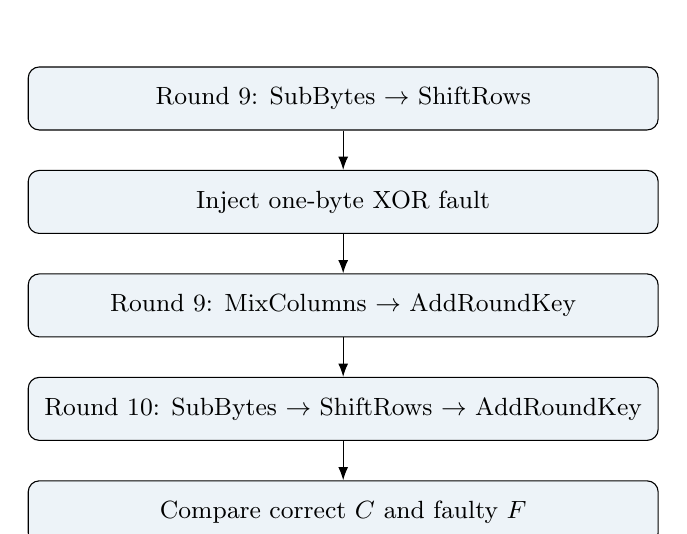
\begin{tikzpicture}[node distance=5mm, every node/.style={font=\small}, box/.style={draw,rounded corners,fill=pale,minimum width=8cm,minimum height=8mm},>=Latex]
\node[box] (a) {Round 9: SubBytes $\to$ ShiftRows};
\node[box,below=of a] (b) {Inject one-byte XOR fault};
\node[box,below=of b] (c) {Round 9: MixColumns $\to$ AddRoundKey};
\node[box,below=of c] (d) {Round 10: SubBytes $\to$ ShiftRows $\to$ AddRoundKey};
\node[box,below=of d] (e) {Compare correct $C$ and faulty $F$};
\foreach \x/\y in {a/b,b/c,c/d,d/e}{\draw[->] (\x)--(\y);}
\end{tikzpicture}\end{center}
\section{Propagation through MixColumns}
If the first byte of a column changes by \(e\), the column difference after MixColumns is
\[\Delta_{MC}=(02e,\ e,\ e,\ 03e)^T.\]
For \(e=\hex{01}\), this is \((\hex{02},\hex{01},\hex{01},\hex{03})^T\). AddRoundKey does not alter XOR differences because both executions use the same round key. The final SubBytes transforms these differences nonlinearly; ShiftRows moves them into separate ciphertext positions.
\section{Which ciphertext bytes are affected?}
For the four round-9 columns, the affected ciphertext positions (in corresponding row order) are:
\begin{center}\begin{tabular}{cc}\toprule Faulted column & Ciphertext byte positions\\\midrule 0&0, 13, 10, 7\\1&4, 1, 14, 11\\2&8, 5, 2, 15\\3&12, 9, 6, 3\\\bottomrule\end{tabular}\end{center}
\section{Constructing candidates for the last AES round key}
For an affected ciphertext position \(j\), and a guessed last-round key byte \(k\), compute
\[d_j(k)=S^{-1}(C_j\xor k)\xor S^{-1}(F_j\xor k).\]
Each byte has 256 candidate values. Four unknown key bytes have \(256^4=2^{32}\) possible combinations before filtering.
Construct a set \(\mathcal D\) containing the MixColumns output differences for a single nonzero faulty byte in any of the four row positions:
\[\mathcal D=\{M(e\mathbf e_r):r\in\{0,1,2,3\},\ e\in\{1,\ldots,255\}\}.\]
This produces \(4\cdot255=1020\) four-byte difference patterns (not 1020 individual bytes). For each proposed key quartet, compute the four \(d_j(k)\) values in their correct \emph{pre-ShiftRows row order} and keep the quartet only if the resulting vector lies in \(\mathcal D\).
\section{Intersecting observations}
A single correct/faulty pair typically leaves multiple candidate key quartets. Repeat with independent faults in the same column and intersect the candidate sets:
\[\mathcal K_{\mathrm{surviving}}=\mathcal K_1\cap\mathcal K_2\cap\cdots.\]
Repeat across all four columns to recover the full 16-byte \(K_{10}\). The notes illustrate candidate filtering using a hypothetical quartet \((\hex{13},\hex{2B},\hex{A7},\hex{17})\); such pedagogical candidate examples should not be confused with a complete independently verified AES fault trace.
\section{Reversing AES-128 key expansion}
Let \(w_0,\ldots,w_{43}\) be 32-bit expanded-key words. For \(i\ge4\),
\[w_i=\begin{cases}w_{i-4}\xor g(w_{i-1}),&i\equiv0\pmod4,\\w_{i-4}\xor w_{i-1},&\text{otherwise},\end{cases}\]
where \(g(w)=\operatorname{SubWord}(\operatorname{RotWord}(w))\xor\operatorname{Rcon}\). In reverse, compute \(w_{i-4}\) by XORing \(w_i\) with the same known right-hand transformation. Begin with \(w_{40},\ldots,w_{43}\) from \(K_{10}\) and work backward to \(w_0,\ldots,w_3\), yielding \(K_0\). No inverse S-box is required for this reversal because the relevant inputs to \(g\) are already known.

\chapter{SM4: Complete Structure and First Round}
\section{Official test vector}
\begin{center}\begin{tabular}{ll}\toprule Plaintext&\hex{0123456789ABCDEFFEDCBA9876543210}\\Master key&\hex{0123456789ABCDEFFEDCBA9876543210}\\Ciphertext&\hex{681EDF34D206965E86B3E94F536E4246}\\\bottomrule\end{tabular}\end{center}
Split the plaintext into four 32-bit words:
\[X_0=\hex{01234567},\quad X_1=\hex{89ABCDEF},\quad X_2=\hex{FEDCBA98},\quad X_3=\hex{76543210}.\]
\section{SM4 round function}
SM4 performs 32 rounds, producing one new 32-bit word per round:
\[\boxed{X_{i+4}=X_i\xor T(X_{i+1}\xor X_{i+2}\xor X_{i+3}\xor rk_i)}.\]
Write \(T=L\circ\tau\), where \(\tau\) substitutes the four bytes through the SM4 S-box and
\[L(B)=B\xor(B\rol2)\xor(B\rol10)\xor(B\rol18)\xor(B\rol24).\]
The output reverses the final four words:
\[C=X_{35}\parallel X_{34}\parallel X_{33}\parallel X_{32}.\]
\section{SM4 key expansion}
The four initial key-schedule words are \(K_i=MK_i\xor FK_i\), with
\[\begin{array}{ll}FK_0=\hex{A3B1BAC6},&FK_1=\hex{56AA3350},\\FK_2=\hex{677D9197},&FK_3=\hex{B27022DC}.\end{array}\]
The key-schedule recurrence is
\[K_{i+4}=K_i\xor T'(K_{i+1}\xor K_{i+2}\xor K_{i+3}\xor CK_i),\quad rk_i=K_{i+4},\]
with \(T'=L'\circ\tau\) and
\[L'(B)=B\xor(B\rol13)\xor(B\rol23).\]
\textbf{Crucial distinction:} encryption uses \(L\), while key expansion uses \(L'\). They have different rotation constants.
For the first round, \(rk_0=\hex{F12186F9}\).
\section{Detailed computation of encryption round 0}
\paragraph{Step 1: XOR the three newest words with the round key.}
\[A=X_1\xor X_2\xor X_3\xor rk_0=\hex{F002C39E}.\]
\paragraph{Step 2: Apply the SM4 S-box to each byte.}
\[\hex{F0}\mapsto\hex{18},\quad\hex{02}\mapsto\hex{E9},\quad\hex{C3}\mapsto\hex{92},\quad\hex{9E}\mapsto\hex{B1}.\]
Thus \(B=\tau(A)=\hex{18E992B1}\).
\paragraph{Step 3: Apply the linear transformation.}
\begin{center}\begin{tabular}{ll}\toprule Term&Hexadecimal value\\\midrule\(B\)&\hex{18E992B1}\\\(B\rol2\)&\hex{63A64AC4}\\\(B\rol10\)&\hex{A64AC463}\\\(B\rol18\)&\hex{4AC463A6}\\\(B\rol24\)&\hex{B118E992}\\\midrule XOR of all five&\hex{26D99622}\\\bottomrule\end{tabular}\end{center}
\paragraph{Step 4: XOR with the oldest word.}
\[X_4=X_0\xor L(B)=\hex{01234567}\xor\hex{26D99622}=\boxed{\hex{27FAD345}}.\]
The next four-word window is \((X_1,X_2,X_3,X_4)\). The following words are \(X_5=\hex{A18B4CB2}\), \(X_6=\hex{11C1E22A}\), and \(X_7=\hex{CC13E2EE}\). After 32 rounds and the output reversal, the official ciphertext is obtained.

\chapter{Differential Fault Analysis of SM4: A Worked Last-Round Model}
\section{Attack model and limitations}
We use a \emph{controlled, known XOR fault} in one byte of the input to the SM4 S-boxes in round 31. This is a pedagogical model, not a claim that a real clock/voltage glitch yields a known XOR value. In this model, all other round inputs remain unchanged.
The last round is
\[X_{35}=X_{31}\xor L(\tau(A)),\qquad A=X_{32}\xor X_{33}\xor X_{34}\xor rk_{31}.\]
The attacker observes the correct ciphertext and a faulty ciphertext. The secret internal values below are supplied \emph{only for checking the simulation}.
\section{Known ciphertext and hidden internal values}
\[\begin{array}{ll}X_{35}=\hex{681EDF34},&X_{34}=\hex{D206965E},\\X_{33}=\hex{86B3E94F},&X_{32}=\hex{536E4246}.\end{array}\]
For this official test vector, the simulation has
\[X_{31}=\hex{7B938F4C},\quad A=\hex{96FF9D45},\quad rk_{31}=\hex{9124A012}.\]
The attacker must recover the key rather than assume it.
\section{Step 1: Inject a known XOR fault}
Alter the first byte of \(A\) by \(e=\hex{01}\):
\[A=\hex{96FF9D45}\longrightarrow A'=\hex{97FF9D45}.\]
\section{Step 2: Observe the S-box difference}
The two S-box outputs are
\[B=\tau(A)=\hex{1A488C73},\qquad B'=\tau(A')=\hex{55488C73}.\]
Consequently,
\[\Delta B=B\xor B'=\hex{4F000000}.\]
\section{Step 3: Propagate the difference through L}
Because \(L\) is XOR-linear,
\[\Delta X_{35}=L(B)\xor L(B')=L(\Delta B)=\hex{734E3D3D}.\]
The correct last word is \(X_{35}=\hex{681EDF34}\), so the faulty last word is
\[X'_{35}=\hex{681EDF34}\xor\hex{734E3D3D}=\hex{1B50E209}.\]
Therefore the attacker sees
\begin{center}\begin{tabular}{ll}\toprule Correct ciphertext&\hex{681EDF34 D206965E 86B3E94F 536E4246}\\Faulty ciphertext&\hex{1B50E209 D206965E 86B3E94F 536E4246}\\Difference&\hex{734E3D3D 00000000 00000000 00000000}\\\bottomrule\end{tabular}\end{center}
\section{Step 4: Undo the linear layer from observed data}
The attacker computes
\[\Delta B=L^{-1}(\Delta X_{35})=L^{-1}(\hex{734E3D3D})=\hex{4F000000}.\]
The first S-box byte therefore satisfies
\[S(a)\xor S(a\xor\hex{01})=\hex{4F}.\]
Enumerating all 256 possible input bytes gives the candidate set
\[\mathcal A_1=\{\hex{96},\hex{97}\}.\]
\section{Step 5: Convert S-box input candidates to key candidates}
The attacker knows the last three words from the ciphertext:
\[X_{32}\xor X_{33}\xor X_{34}=\hex{07DB3D57}.\]
Since \(rk_{31}=A\xor\hex{07DB3D57}\), the first byte of the key is
\[rk_{31}[0]=a\xor\hex{07}.\]
Thus \(a=\hex{96}\) yields \(\hex{91}\), while \(a=\hex{97}\) yields \(\hex{90}\). After one observation, the candidates are \(\{\hex{91},\hex{90}\}\).
\section{Step 6: Use independent observations}
Repeat with the \emph{same plaintext and state}, but use a known XOR fault \(e=\hex{02}\). The new S-box difference is \(d_2=\hex{81}\). Keep only input candidates satisfying both
\[\begin{cases}S(a)\xor S(a\xor\hex{01})=\hex{4F},\\S(a)\xor S(a\xor\hex{02})=\hex{81}.\end{cases}\]
The intersection identifies \(a=\hex{96}\), hence \(rk_{31}[0]=\hex{91}\).
\section{Step 7: Repeat for the other three bytes}
The supplied worked example reports the following bytewise observations under the same controlled-fault assumption:
\begin{center}\begin{tabular}{ccccc}\toprule Byte&\(d\) for \(e=01\)&\(d\) for \(e=02\)&Recovered \(A\)&Recovered \(rk_{31}\)\\\midrule0&4F&81&96&91\\1&71&83&FF&24\\2&79&6F&9D&A0\\3&80&C9&45&12\\\bottomrule\end{tabular}\end{center}
This reconstructs
\[A=\hex{96FF9D45},\qquad rk_{31}=A\xor\hex{07DB3D57}=\boxed{\hex{9124A012}}.\]
\note{This illustrates last-round subkey recovery \emph{conditional on the fault model}. The listed observations should be validated against a software implementation before treating them as experimental results.}
\section{What happens after recovering the last subkey?}
Knowing \(rk_{31}\), reconstruct the previous state word:
\[X_{31}=X_{35}\xor T(X_{32}\xor X_{33}\xor X_{34}\xor rk_{31}).\]
For the example, \(X_{31}=\hex{7B938F4C}\). However, this does \emph{not} automatically reveal \(rk_{30}\). Additional fault observations and state constraints are required for rounds 30, 29, and 28. The present worked example does not demonstrate that stage of the attack.

\chapter{SM4: Recovering the Master Key from Four Round Keys}
\section{Required subkeys}
If four consecutive final subkeys have been recovered, then
\begin{center}\begin{tabular}{cc}\toprule Key-schedule word&Round key\\\midrule\(K_{32}\)&\(rk_{28}=\hex{428D3654}\)\\\(K_{33}\)&\(rk_{29}=\hex{62293496}\)\\\(K_{34}\)&\(rk_{30}=\hex{01CF72E5}\)\\\(K_{35}\)&\(rk_{31}=\hex{9124A012}\)\\\bottomrule\end{tabular}\end{center}
These are reference subkeys from the official example; \emph{only} \(rk_{31}\) was recovered in the preceding pedagogical DFA walkthrough. Chapter~\ref{chap:all-attacks-code} explains how the current code actually recovers all four subkeys with a selectable-round fault oracle.
\section{Reverse the recurrence}
The forward key schedule is
\[K_{i+4}=K_i\xor T'(K_{i+1}\xor K_{i+2}\xor K_{i+3}\xor CK_i).\]
XOR is self-inverse, so
\[\boxed{K_i=K_{i+4}\xor T'(K_{i+1}\xor K_{i+2}\xor K_{i+3}\xor CK_i)}.\]
Start with \(i=31\), then decrease to \(i=0\). For example,
\[K_{31}=K_{35}\xor T'(K_{32}\xor K_{33}\xor K_{34}\xor CK_{31}),\]
where \(CK_{31}=\hex{646B7279}\). This yields the previous expanded-key word \(K_{31}=\hex{F1780C81}\) in the official test vector. Continue to recover \(K_0,K_1,K_2,K_3\).
\section{Undo the initial constants}
Finally,
\[MK_i=K_i\xor FK_i\qquad(i=0,1,2,3),\]
and concatenate the four master-key words:
\[\boxed{MK=\hex{0123456789ABCDEFFEDCBA9876543210}}.\]

\chapter{Giraud Fault Attack on AES-128 and Its Adaptation to SM4}
\label{chap:giraud}
\section{Core idea and comparison with Piret--Quisquater}
Giraud's AES fault-analysis approach exploits a \emph{single-bit} fault close to the last round. In contrast to the Piret--Quisquater example, which injects a byte fault before the ninth-round MixColumns and typically modifies four ciphertext bytes, a single-byte fault immediately before the final SubBytes affects only one ciphertext byte: the last AES round does not contain MixColumns. The attacker tests last-round key-byte candidates by checking whether the inverse-S-box input difference has Hamming weight one.

\section{AES-128: precise fault location}
Let $U$ denote the state after round 9 AddRoundKey, just before round 10 SubBytes. A one-bit XOR fault modifies a single input byte $a$ into $a'=a\xor e$, where $e\in\{\hex{01},\hex{02},\hex{04},\hex{08},\hex{10},\hex{20},\hex{40},\hex{80}\}$. Round 10 performs SubBytes, ShiftRows and AddRoundKey $K_{10}$; there is no MixColumns. ShiftRows relocates the changed byte without increasing the number of affected bytes.

For the affected ciphertext position $j$, with correct byte $c$, faulty byte $f$, and unknown last-round key byte $k$, the attacker evaluates
\begin{equation}
\delta(k)=S_{\mathrm{AES}}^{-1}(c\xor k)\xor S_{\mathrm{AES}}^{-1}(f\xor k).
\label{eq:giraud_aes_test}
\end{equation}
The candidate is compatible with the fault model if
\begin{equation}
\delta(k)\in\mathcal E=\{\hex{01},\hex{02},\hex{04},\hex{08},\hex{10},\hex{20},\hex{40},\hex{80}\}.
\end{equation}
Equivalently, the 8-bit value $\delta(k)$ must have Hamming weight exactly one. If the injected bit position is known, the condition can be made stronger: $\delta(k)=e$.

\section{Worked AES-128 example: the first ciphertext byte}
We use the official AES-128 test vector already introduced in this report:
\begin{align*}
P&=\hex{00112233445566778899AABBCCDDEEFF},\\
K_0&=\hex{000102030405060708090A0B0C0D0E0F},\\
C&=\hex{69C4E0D86A7B0430D8CDB78070B4C55A}.
\end{align*}
The first byte entering the final SubBytes is $a=\hex{BD}$. Inject $e=\hex{01}$ in that byte:
\begin{equation}
\hex{BD}\xor\hex{01}=\hex{BC}.
\end{equation}
The AES S-box maps $S(\hex{BD})=\hex{7A}$ and $S(\hex{BC})=\hex{65}$. The first byte of $K_{10}$ is $\hex{13}$, so
\begin{align*}
c&=\hex{7A}\xor\hex{13}=\hex{69},\\
f_1&=\hex{65}\xor\hex{13}=\hex{76}.
\end{align*}
Thus the simulated faulty ciphertext is
\begin{equation}
F_1=\hex{76C4E0D86A7B0430D8CDB78070B4C55A}.
\end{equation}
The attacker does not assume the value $\hex{13}$: it is shown here solely to verify the example. For candidate $k=\hex{13}$, equation~\eqref{eq:giraud_aes_test} gives
\begin{align*}
S^{-1}(\hex{69}\xor\hex{13})&=S^{-1}(\hex{7A})=\hex{BD},\\
S^{-1}(\hex{76}\xor\hex{13})&=S^{-1}(\hex{65})=\hex{BC},\\
\delta(\hex{13})&=\hex{BD}\xor\hex{BC}=\boxed{\hex{01}}.
\end{align*}
The candidate is compatible with a single-bit fault, but one correct/faulty pair may leave several candidates.

\section{Multiple faults and candidate intersection}
Repeat the encryption with the same plaintext and key and introduce an independent single-bit fault at the same location. In the worked example, choosing $e_2=\hex{02}$ produces $a_2'=\hex{BF}$ and a second faulty first ciphertext byte $f_2=\hex{1B}$. For observation $t$, define
\begin{equation}
\mathcal K_t=\bigl\{k\in\{0,\ldots,255\}:S^{-1}(c\xor k)\xor S^{-1}(f_t\xor k)\in\mathcal E\bigr\}.
\end{equation}
The surviving candidates are the intersection $\mathcal K=\bigcap_t\mathcal K_t$. For the illustrated pair of faults, the recovered first byte is $K_{10}[0]=\hex{13}$. The number of observations required is not fixed: it depends on the fault model and the observed differences.

Repeating the experiment across all sixteen pre-final-SubBytes byte positions allows the attacker, under this model, to reconstruct all sixteen bytes of $K_{10}$. For the official vector,
\begin{equation}
K_{10}=\hex{13111D7FE3944A17F307A78B4D2B30C5}.
\end{equation}
The AES-128 key schedule can then be reversed to recover the original key $K_0$, as explained in the preceding AES key-expansion chapter.

\section{Adaptation of the single-bit idea to SM4}
\label{sec:giraud_sm4}
The corresponding SM4 experiment is an \emph{adaptation of the single-bit differential filtering principle}, rather than a claim that the original AES attack transfers unchanged. The SM4 last round is
\begin{equation}
X_{35}=X_{31}\xor L\bigl(\tau(A)\bigr),\qquad A=X_{32}\xor X_{33}\xor X_{34}\xor rk_{31}.
\end{equation}
The output is $C=(X_{35},X_{34},X_{33},X_{32})$. Inject a single-bit fault in one byte of $A$, just before the last-round S-boxes. Unlike AES, the SM4 linear map $L$ diffuses the one-byte S-box output difference over the 32-bit word $X_{35}$. The other three ciphertext words remain unchanged \emph{under the assumed isolated-fault model}.

Let $F$ be the faulty ciphertext and $\Delta X_{35}=X_{35}\xor X'_{35}$. Since $L$ is linear and invertible, the attacker can compute
\begin{equation}
\Delta B=L^{-1}(\Delta X_{35})=\tau(A)\xor\tau(A').
\end{equation}
For an affected byte with S-box input $a$ and unknown single-bit error $e$, candidate inputs satisfy
\begin{equation}
S_{\mathrm{SM4}}(a)\xor S_{\mathrm{SM4}}(a\xor e)=d,
\quad e\in\mathcal E,
\end{equation}
where $d$ is the corresponding byte of $\Delta B$. If $e$ is known from the simulation, it is used directly; otherwise all eight one-bit masks must be tested. Multiple correct/faulty observations reduce the candidate set by intersection.

\section{Worked SM4 example and recovery of $rk_{31}$}
Using the official SM4 test vector,
\begin{align*}
P&=\hex{0123456789ABCDEFFEDCBA9876543210},\\
MK&=\hex{0123456789ABCDEFFEDCBA9876543210},\\
C&=\hex{681EDF34D206965E86B3E94F536E4246},
\end{align*}
the simulated input of the last S-box layer is $A=\hex{96FF9D45}$. A one-bit fault $e=\hex{01000000}$ gives $A'=\hex{97FF9D45}$. The substitution outputs are
\begin{align*}
\tau(A)&=\hex{1A488C73},\\
\tau(A')&=\hex{55488C73},\\
\Delta B&=\hex{4F000000}.
\end{align*}
After the linear layer,
\begin{equation}
\Delta X_{35}=L(\hex{4F000000})=\hex{734E3D3D}.
\end{equation}
Therefore the faulty output is
\begin{equation}
F_1=\hex{1B50E209D206965E86B3E94F536E4246}.
\end{equation}
From the observed difference alone, the attacker obtains $\Delta B=L^{-1}(\hex{734E3D3D})=\hex{4F000000}$. With known fault mask $\hex{01}$ in the first byte, the candidate equation is
\begin{equation}
S_{\mathrm{SM4}}(a)\xor S_{\mathrm{SM4}}(a\xor\hex{01})=\hex{4F}.
\end{equation}
The first observation permits $a\in\{\hex{96},\hex{97}\}$. A second simulated fault of mask $\hex{02}$ gives the first-byte S-box difference $\hex{81}$. Intersecting both sets identifies $a=\hex{96}$.

The three known ciphertext words yield
\begin{equation}
X_{32}\xor X_{33}\xor X_{34}=\hex{07DB3D57}.
\end{equation}
Thus the first last-round key byte is
\begin{equation}
rk_{31}[0]=\hex{96}\xor\hex{07}=\boxed{\hex{91}}.
\end{equation}
The supplied worked example applies analogous observations to the remaining three S-box inputs, obtaining
\begin{equation}
A=\hex{96FF9D45},\qquad rk_{31}=A\xor\hex{07DB3D57}=\boxed{\hex{9124A012}}.
\end{equation}
The bytewise simulated differences are summarized below.
\begin{center}
\begin{tabular}{ccccc}\toprule
Byte&$d$ for $e=01$&$d$ for $e=02$&Recovered $A$&Recovered $rk_{31}$\\\midrule
0&4F&81&96&91\\
1&71&83&FF&24\\
2&79&6F&9D&A0\\
3&80&C9&45&12\\\bottomrule
\end{tabular}
\end{center}
\note{The numerical values in this subsection are simulated, not physical fault-injection measurements. In particular, knowledge of the exact XOR mask is a strong experimental assumption.}

\section{From the final SM4 subkey to the master key}
Recovering $rk_{31}$ is not equivalent to recovering the 128-bit master key. The SM4 key schedule needs four consecutive 32-bit round keys to be inverted. In the official test vector these are
\begin{align*}
rk_{28}&=\hex{428D3654},&rk_{29}&=\hex{62293496},\\
rk_{30}&=\hex{01CF72E5},&rk_{31}&=\hex{9124A012}.
\end{align*}
The values $rk_{28}$, $rk_{29}$ and $rk_{30}$ are \emph{reference values}, not keys shown to have been recovered by the two last-round faults. The two last-round faults do not recover these other keys. The implemented multi-round extension in Chapter~\ref{chap:all-attacks-code} obtains them by requesting new faults in rounds 30, 29 and 28 and undoing previously recovered later rounds.

With four consecutive round keys, set $K_{i+4}=rk_i$ and invert the SM4 recurrence:
\begin{equation}
K_i=K_{i+4}\xor T'\bigl(K_{i+1}\xor K_{i+2}\xor K_{i+3}\xor CK_i\bigr).
\end{equation}
Iterating backward yields $K_0,K_1,K_2,K_3$. Undo the fixed initial constants $FK_i$ via $MK_i=K_i\xor FK_i$ and concatenate the four words to recover the 128-bit master key.

\section{Experimental implications}
A software simulation can inject an exact XOR mask at a chosen intermediate value. On an STM32 target, a voltage or clock glitch may instead alter multiple bits, skip an instruction, affect control flow, or produce no useful fault. A practical evaluation should therefore log correct and faulty ciphertexts, classify observed fault patterns, verify whether the assumed location and single-bit model are plausible, and report recovery success separately from simulation-only results.

\chapter{AES versus SM4: Key Lessons}
\begin{center}\begin{tabular}{p{.35\linewidth}p{.28\linewidth}p{.28\linewidth}}\toprule Property&AES-128&SM4\\\midrule Block size&128 bits&128 bits\\Key size&128 bits&128 bits\\Rounds&10&32\\State&4$\times$4 byte matrix&Four 32-bit words\\Nonlinearity&AES S-box&SM4 S-box\\Linear diffusion&MixColumns and ShiftRows&Rotations and XOR in \(L\)\\Last-round target&\(K_{10}\), 128 bits&\(rk_{31}\), 32 bits\\Master-key recovery&Reverse AES expansion&Reverse SM4 expansion from four consecutive round keys\\\bottomrule\end{tabular}\end{center}
\section*{Summary}
For AES Giraud, inject a one-bit fault before final-round SubBytes, test inverse-S-box differences for Hamming weight one, and intersect key-byte candidates. The corresponding SM4 adaptation first inverts the linear map $L$ to isolate the S-box differential.

For AES Piret--Quisquater, compare correct and faulty ciphertexts, invert the last S-box under candidate \(K_{10}\) bytes, match round-9 MixColumns differential patterns, intersect candidates, and reverse the AES key schedule.

For the illustrated SM4 model, compare correct and faulty ciphertexts, invert the linear map \(L\), test S-box input candidates using the known fault differences, derive \(rk_{31}\), and obtain further subkeys with additional appropriate experiments. Once four consecutive round keys are known, the SM4 key schedule can be reversed exactly.


\chapter{Python Implementation and Reproducible Terminal Results}
\label{chap:implementation}
This chapter connects the preceding mathematical derivations to the actual Python project provided with this report. The listings below are \emph{excerpts of the project source files}, not pseudocode. The console blocks were captured by executing the supplied scripts on 24 October 2026. These are software simulations with a controllable fault observer, not physical STM32 measurements.

\section{Repository structure and execution}
The principal modules are \texttt{aes.py} (AES operations), \texttt{sm4.py} (SM4 operations), \texttt{piret.py} (DFA and round peeling), \texttt{giraud.py} (single-bit candidate filtering), and \texttt{run.py} (combined demonstration). The repository stores these modules in \texttt{src/}; \texttt{src/gui.py} provides the interactive interface. The commands below are run from the repository root.
\begin{lstlisting}[style=terminal]
python src/giraud.py --algorithm aes --known-bit
python src/giraud.py --algorithm sm4 --known-bit
python src/piret.py --algorithm sm4
\end{lstlisting}
The project also supports an unknown-bit model by omitting \texttt{--known-bit}. The \texttt{--known-bit} option is used for the reproducible outputs reproduced here.

\section{AES-128 implementation: S-box, diffusion, and key expansion}
The following code implements AES finite-field multiplication and column mixing. This is the operation responsible for the characteristic four-byte differential exploited by Piret--Quisquater.
\begin{lstlisting}[style=pycode,caption={AES finite-field arithmetic, from aes.py}]
def xtime(a):
    """Multiply a byte by x (02) in GF(2^8), reducing by polynomial 0x11B."""
    result = a << 1

    # If the x^8 term overflows, reduction contributes 0x1B to the low byte.
    if a & 0x80:
        result ^= 0x1B

    return result & 0xFF


def gf_mul(a, b):
    """Multiply bytes in the AES field; field addition is XOR, not integer +."""
    result = 0

    for _ in range(8):
        if b & 1:
            result ^= a

        # Shift-and-add multiplication, using xtime for polynomial reduction.
        a = xtime(a)
        b >>= 1

    return result


# ============================================================================
# 5. ROUND TRANSFORMATIONS: ALL MATRIX OPERATIONS ARE IN PLACE
# ============================================================================
\end{lstlisting}
\begin{lstlisting}[style=pycode,caption={AES MixColumns, from aes.py}]
def mix_column(column):
    """Return M * column in GF(2^8), without modifying the four input bytes.

    Copying a column before mixing matters: every output byte must use the same
    original input, never a value already overwritten earlier in the operation.
    """
    result = []
    for coefficients in MIX_MATRIX:
        value = 0
        for coefficient, byte in zip(coefficients, column):
            value ^= gf_mul(coefficient, byte)
        result.append(value)
    return result


def mix_columns(state):
    """Mix each column in place; the normal algorithm never prints output."""
    for column in range(4):
        mixed = mix_column([state[row][column] for row in range(4)])
        for row in range(4):
            state[row][column] = mixed[row]
\end{lstlisting}
\begin{lstlisting}[style=pycode,caption={AES round-key expansion, from aes.py}]
def key_expansion(key):
    """Expand the 16-byte master key into eleven independent round-key matrices.

    Each new word XORs the word four positions back with the previous word.
    Every fourth word first applies RotWord, SubWord and the round constant.
    """
    validate_block(key, "AES-128 key")
    # Four initial words become 44 words: K0 plus ten encryption round keys.
    words = [list(key[4 * i:4 * i + 4]) for i in range(4)]

    for i in range(4, 4 * (N_ROUNDS + 1)):
        temp = words[i - 1].copy()

        if i % 4 == 0:
            # Rcon changes only the first byte of the transformed key word.
            temp = sub_word(rot_word(temp))
            temp[0] ^= RCON[i // 4]

        new_word = [words[i - 4][j] ^ temp[j] for j in range(4)]

        words.append(new_word)

    round_keys = []

    for round_number in range(N_ROUNDS + 1):
        # Convert four consecutive words into the same layout as the data state.
        key_bytes = []

        for i in range(4):
            key_bytes.extend(words[round_number * 4 + i])

        round_keys.append(bytes_to_state(key_bytes))

    return round_keys


# ============================================================================
# 7. NORMAL ENCRYPTION / DECRYPTION AND OPTIONAL EXTERNAL OBSERVATION
# ============================================================================
\end{lstlisting}

\section{SM4 implementation: rotations, S-boxes, and 32 rounds}
The SM4 code keeps the encryption diffusion $L$ distinct from the key-schedule diffusion $L'$. The observer hook allows the test harness to modify an intermediate value at a chosen round.
\begin{lstlisting}[style=pycode,caption={SM4 rotations, diffusion, and substitution, from sm4.py}]
def rotl(val: int, count: int) -> int:
    """Rotate a 32-bit unsigned word left; overflow wraps into the low bits."""
    return ((val << count) & WORD_MASK) | (val >> (32 - count))


def linear(b: int) -> int:
    """Data diffusion L: XOR the word with rotations by 2, 10, 18 and 24.

    L is XOR-linear: L(a XOR b) = L(a) XOR L(b). The SM4 DFA uses this
    property to invert an observed output difference before testing the S-box.
    """
    return b ^ rotl(b, 2) ^ rotl(b, 10) ^ rotl(b, 18) ^ rotl(b, 24)


def linear_key(b: int) -> int:
    """Key-schedule diffusion L-prime: rotations 13 and 23, not data-map L."""
    return b ^ rotl(b, 13) ^ rotl(b, 23)


def sbox(a: int) -> int:
    """Apply tau: substitute all four bytes, preserving big-endian word order."""
    input_bytes = struct.pack('>I', a)
    substituted_bytes = bytes(SBOX[byte] for byte in input_bytes)
    return struct.unpack('>I', substituted_bytes)[0]


# ============================================================================
# 4. SINGLE-ROUND RECURRENCES
# ============================================================================
\end{lstlisting}
\begin{lstlisting}[style=pycode,caption={SM4 round function and round-key generation, from sm4.py}]
def round(x: list[int], rk: int, observer=None, round_index=0):
    """Return the next rolling window without modifying the supplied words.

    A = X[i+1] XOR X[i+2] XOR X[i+3] XOR rk[i]
    X[i+4] = X[i] XOR L(tau(A))
    """
    sbox_input = observe(observer, round_index, "Sbox input", x[1] ^ x[2] ^ x[3] ^ rk)
    substituted = observe(observer, round_index, "Sbox output", sbox(sbox_input))
    diffused = observe(observer, round_index, "Linear output", linear(substituted))
    new_word = observe(observer, round_index, "New word", x[0] ^ diffused)
    return x[1], x[2], x[3], new_word


def generate_round_key(k: list[int], round: int) -> int:
    """Compute K[i+4] from four consecutive schedule words and CK[i].

    The parameter name round is retained for callers using keyword arguments.
    Encryption and expansion share tau, but expansion must use linear_key.
    """
    return k[0] ^ linear_key(sbox(k[1] ^ k[2] ^ k[3] ^ CK[round]))


# ============================================================================
# 5. KEY EXPANSION: FOUR MASTER WORDS TO 32 ROUND KEYS
# ============================================================================


def key_expansion(key: bytes) -> list[int]:
    """Return rk0..rk31; each is one new word from the key recurrence."""
    if len(key) != BLOCK_SIZE:
        raise ValueError("SM4 key must contain exactly 16 bytes.")
    master_words = struct.unpack(">4I", key)
    schedule_words = [master_words[i] ^ FK[i] for i in range(4)]

    for i in range(N_ROUNDS):
        # Keep previous words for readability; the recurrence consumes a window.
        next_key = generate_round_key(schedule_words[i:i+4], i)
        schedule_words.append(next_key)

    # The initial four whitened words are not encryption round keys.
    return schedule_words[4:]


# ============================================================================
# 6. SHARED BLOCK PROCESSING AND PUBLIC ENCRYPT/DECRYPT WRAPPERS
# ============================================================================
\end{lstlisting}

\section{AES Giraud: filtering last-round key candidates}
For each possible final-round key byte, the implementation undoes the final AddRoundKey and S-box, and tests whether the recovered input difference is a single bit. The solver does not receive the master key.
\begin{lstlisting}[style=pycode,caption={AES Giraud candidate test, from giraud.py}]
def aes_candidates(correct, faulty, known_mask=None):
    """Return the affected output position and its compatible K10 byte values.

    For each guess k:
      delta = InvSbox[C[j] XOR k] XOR InvSbox[F[j] XOR k]
    Keep k when delta has exactly one set bit, or equals the known bit mask.
    """
    aes.validate_block(correct, "Correct ciphertext")
    aes.validate_block(faulty, "Faulty ciphertext")
    if known_mask is not None:
        validate_mask(known_mask)

    # Without final-round MixColumns, only one ciphertext byte should change.
    changed = [index for index in range(16) if correct[index] != faulty[index]]
    if len(changed) != 1:
        raise ValueError("AES Giraud requires exactly one changed ciphertext byte.")
    position = changed[0]
    allowed = SINGLE_BITS if known_mask is None else (known_mask,)

    candidates = set()
    for guess in range(256):
        clean_input = AES_INVERSE_SBOX[correct[position] ^ guess]
        faulty_input = AES_INVERSE_SBOX[faulty[position] ^ guess]
        difference = clean_input ^ faulty_input
        if difference in allowed:
            candidates.add(guess)
    return position, candidates
\end{lstlisting}
\subsection{Observed AES terminal output}
The following excerpt is from an actual execution of \texttt{python src/giraud.py --algorithm aes --known-bit}. It shows the filtering process and final verification.
\begin{lstlisting}[style=terminal,caption={Recorded AES Giraud execution excerpt}]

============================================================================
GIRAUD / AES-128
Correct ciphertext: 69C4E0D86A7B0430D8CDB78070B4C55A
Bit known to solver: True
AES: require HW(InvSbox[C XOR k] XOR InvSbox[F XOR k]) = 1.

Key byte 0, observation 1, simulator mask 01
Correct: 69 C4 E0 D8 6A 7B 04 30 D8 CD B7 80 70 B4 C5 5A
Faulty:  76 C4 E0 D8 6A 7B 04 30 D8 CD B7 80 70 B4 C5 5A
XOR:     1F 00 00 00 00 00 00 00 00 00 00 00 00 00 00 00
Candidate count: 256 -> 4
Survivors: 0A 0C 13 15

Key byte 0, observation 2, simulator mask 02
Correct: 69 C4 E0 D8 6A 7B 04 30 D8 CD B7 80 70 B4 C5 5A
Faulty:  1B C4 E0 D8 6A 7B 04 30 D8 CD B7 80 70 B4 C5 5A
XOR:     72 00 00 00 00 00 00 00 00 00 00 00 00 00 00 00
Candidate count: 4 -> 1
Survivors: 13

Key byte 13, observation 1, simulator mask 01
Correct: 69 C4 E0 D8 6A 7B 04 30 D8 CD B7 80 70 B4 C5 5A
Faulty:  69 C4 E0 D8 6A 7B 04 30 D8 CD B7 80 70 83 C5 5A
XOR:     00 00 00 00 00 00 00 00 00 00 00 00 00 37 00 00
Candidate count: 256 -> 2
Survivors: 1C 2B

Key byte 13, observation 2, simulator mask 02
Correct: 69 C4 E0 D8 6A 7B 04 30 D8 CD B7 80 70 B4 C5 5A
Faulty:  69 C4 E0 D8 6A 7B 04 30 D8 CD B7 80 70 7B C5 5A
XOR:     00 00 00 00 00 00 00 00 00 00 00 00 00 CF 00 00

... [intermediate observations omitted from this printed excerpt]

XOR:     00 00 00 9A 00 00 00 00 00 00 00 00 00 00 00 00
Candidate count: 2 -> 1
Survivors: 7F

Recovered K10: 13111D7FE3944A17F307A78B4D2B30C5
Recovered master key: 000102030405060708090A0B0C0D0E0F
Verification: PASS / 32 faulty outputs
\end{lstlisting}

\section{SM4 Giraud-inspired filtering}
SM4 requires an extra step: invert the linear transformation $L$ to isolate the S-box output difference. The following code tests candidate S-box inputs, then translates them into candidates for a byte of the last-round subkey using the three unchanged state words.
\begin{lstlisting}[style=pycode,caption={SM4 S-box differential candidate filter, from giraud.py}]
def sm4_candidates(correct, faulty, known_mask=None):
    """Return affected byte, round-key guesses, input guesses and DeltaB.

    Inputs may be actual final ciphertexts or peeled views at an earlier round.

    1. Observe DeltaX35 from the first output word.
    2. Undo linear diffusion: DeltaB = L-inverse(DeltaX35).
    3. Keep a if S(a) XOR S(a XOR e) matches the observed byte difference.
    4. Convert a into a key guess using the three unchanged output words.
    """
    aes.validate_block(correct, "Correct ciphertext")
    aes.validate_block(faulty, "Faulty ciphertext")
    if known_mask is not None:
        validate_mask(known_mask)

    # SM4 outputs X35 || X34 || X33 || X32; only X35 may change in this model.
    if correct[4:] != faulty[4:]:
        raise ValueError("SM4 last-round model requires three output words unchanged.")
    delta_x35 = int.from_bytes(correct[:4], "big") ^ int.from_bytes(faulty[:4], "big")
    delta_b = inverse_linear(delta_x35)
    differences = delta_b.to_bytes(4, "big")
    changed = [index for index in range(4) if differences[index] != 0]
    if len(changed) != 1:
        raise ValueError("SM4 inverse-L difference must affect one S-box byte.")
    position = changed[0]
    allowed = SINGLE_BITS if known_mask is None else (known_mask,)

    # The input value a is unknown. Test every value against each permitted bit.
    inputs = set()
    for guess in range(256):
        for error in allowed:
            difference = sm4.SBOX[guess] ^ sm4.SBOX[guess ^ error]
            if difference == differences[position]:
                inputs.add(guess)
                break

    # A = X32 XOR X33 XOR X34 XOR rk31; all three data words are observable.
    x34 = int.from_bytes(correct[4:8], "big")
    x33 = int.from_bytes(correct[8:12], "big")
    x32 = int.from_bytes(correct[12:16], "big")
    known_byte = ((x32 ^ x33 ^ x34) >> (24 - 8 * position)) & 0xFF
    candidates = {guess ^ known_byte for guess in inputs}
    return position, candidates, inputs, delta_b
\end{lstlisting}
\subsection{Observed SM4 terminal output}
The first fault produces a 32-bit ciphertext difference; the inverse-linear operation reduces it to a one-byte S-box difference. A second independent observation reduces the key-byte candidates from two to one.
\begin{lstlisting}[style=terminal,caption={Recorded SM4 Giraud-inspired execution excerpt}]

============================================================================
GIRAUD-INSPIRED / SM4
Correct ciphertext: 681EDF34D206965E86B3E94F536E4246
Bit known to solver: True
SM4: invert L, then test S(a) XOR S(a XOR e) for one-bit errors.

Round 31, key byte 0, observation 1
Correct: 68 1E DF 34 D2 06 96 5E 86 B3 E9 4F 53 6E 42 46
Faulty:  1B 50 E2 09 D2 06 96 5E 86 B3 E9 4F 53 6E 42 46
XOR:     73 4E 3D 3D 00 00 00 00 00 00 00 00 00 00 00 00
Undo recovered later rounds: {}
Correct: 68 1E DF 34 D2 06 96 5E 86 B3 E9 4F 53 6E 42 46
Faulty:  1B 50 E2 09 D2 06 96 5E 86 B3 E9 4F 53 6E 42 46
XOR:     73 4E 3D 3D 00 00 00 00 00 00 00 00 00 00 00 00
Candidates: 256 -> 2

Round 31, key byte 0, observation 2
Correct: 68 1E DF 34 D2 06 96 5E 86 B3 E9 4F 53 6E 42 46
Faulty:  ED 9D D9 32 D2 06 96 5E 86 B3 E9 4F 53 6E 42 46
XOR:     85 83 06 06 00 00 00 00 00 00 00 00 00 00 00 00
Undo recovered later rounds: {}
Correct: 68 1E DF 34 D2 06 96 5E 86 B3 E9 4F 53 6E 42 46
Faulty:  ED 9D D9 32 D2 06 96 5E 86 B3 E9 4F 53 6E 42 46
XOR:     85 83 06 06 00 00 00 00 00 00 00 00 00 00 00 00
Candidates: 2 -> 1

Round 31, key byte 1, observation 1
Correct: 68 1E DF 34 D2 06 96 5E 86 B3 E9 4F 53 6E 42 46
Faulty:  AD AB AF F1 D2 06 96 5E 86 B3 E9 4F 53 6E 42 46
XOR:     C5 B5 70 C5 00 00 00 00 00 00 00 00 00 00 00 00
Undo recovered later rounds: {}

... [intermediate observations omitted from this printed excerpt]

Candidates: 2 -> 1
Recovered rk31: 9124A012
Recovered rk30: 01CF72E5
Recovered rk29: 62293496
Recovered rk28: 428D3654
Recovered master key: 0123456789ABCDEFFEDCBA9876543210
Verification: PASS / 32 faulty outputs / no reference subkeys
\end{lstlisting}

\section{Recovering SM4 rounds 31 through 28}
The source project implements an additional \emph{multi-round simulated attack}, beyond the last-round example described earlier in this report. Once $rk_{31}$ is recovered, its value is used to undo the last round in both correct and faulty ciphertexts. A separate controlled fault at round 30 can then be analyzed as a last-round differential on the reconstructed state. The same process is repeated for rounds 29 and 28.

Crucially, the algorithm does \emph{not} supply reference round keys to the recovery function. It uses previously recovered keys to peel later rounds. However, its fault oracle must be capable of injecting faults at each of the four targeted rounds, a strong capability not established by these software tests on physical hardware.
\begin{lstlisting}[style=pycode,caption={Undoing already recovered SM4 rounds, from piret.py}]
def peel_sm4(ciphertext, target_round, recovered_keys):
    """Undo only rounds whose subkeys have ALREADY been recovered by DFA.

    Return a reversed four-word output at the end of target_round. This lets
    the same last-round equations analyze rounds 30, 29 and 28 in succession.
    No reference round keys or secret intermediate values are accepted.
    """
    aes.validate_block(ciphertext, "SM4 ciphertext")
    if not 28 <= target_round <= 31:
        raise ValueError("Full SM4 recovery targets rounds 28..31.")
    words = list(struct.unpack(">4I", ciphertext))[::-1]
    for number in range(31, target_round, -1):
        if number not in recovered_keys:
            raise ValueError(f"Cannot undo round {number} before recovering its subkey.")
        previous = words[3] ^ sm4.linear(sm4.sbox(words[0] ^ words[1] ^ words[2] ^ recovered_keys[number]))
        words = [previous, words[0], words[1], words[2]]
    return struct.pack(">4I", *words[::-1])
\end{lstlisting}
\begin{lstlisting}[style=pycode,caption={Sequential recovery of four SM4 subkeys, from piret.py}]
def recover_sm4_master_key(correct, fault_oracle, masks=(1, 2, 3, 4, 5, 6, 7, 8), start_byte=0, candidate_filter=None, observer=None):
    """Recover rk31 -> rk28 and reverse the schedule, using outputs only.

    fault_oracle(round, byte, mask) returns a faulty ciphertext. It represents
    a target capable of a controlled fault in EACH of the final four rounds.
    The solver receives no master key, schedule, or reference subkeys.
    The default filter uses known masks; Giraud supplies its single-bit filter.
    """
    aes.validate_block(correct, "Correct SM4 ciphertext")
    masks = tuple(masks)
    if not masks or len(set(masks)) != len(masks) or any(not 1 <= mask <= 255 for mask in masks) or not 0 <= start_byte < 4:
        raise ValueError("Use distinct nonzero byte masks and start_byte 0..3.")
    keys, history, counts, used = {}, [], {}, 0
    for number in range(31, 27, -1):
        clean_view = peel_sm4(correct, number, keys)
        subkey = bytearray(4)
        for byte in [(start_byte + offset) % 4 for offset in range(4)]:
            survivors = None
            for observation, mask in enumerate(masks, 1):
                faulty = bytes(fault_oracle(number, byte, mask))
                faulty_view = peel_sm4(faulty, number, keys)
                if candidate_filter is None:
                    fresh, inputs, delta = sm4_byte_candidates(clean_view, faulty_view, byte, mask)
                else:
                    position, fresh, inputs, delta = candidate_filter(clean_view, faulty_view, mask)
                    if position != byte:
                        raise ValueError("Fault observation does not match the requested byte.")
                before = 256 if survivors is None else len(survivors)
                survivors = set(fresh) if survivors is None else survivors & fresh
                if not survivors:
                    raise ValueError("SM4 candidate intersection is empty; fault model is incompatible.")
                used += 1
                counts[f"{number}:{byte}"] = len(survivors)
                event = dict(round=number, byte=byte, observation=observation, mask=mask, before=before, pair_candidates=len(fresh), remaining=len(survivors), survivors=sorted(survivors), inputs=sorted(inputs), delta_b=delta, correct=correct.hex(), faulty=faulty.hex(), clean_view=clean_view.hex(), faulty_view=faulty_view.hex(), peeled_with={str(i): f"{value:08X}" for i, value in keys.items()})
                history.append(event)
                if observer is not None:
                    observer(dict(event))
                if len(survivors) == 1:
                    subkey[byte] = next(iter(survivors))
                    break
            else:
                return dict(master_key=None, round_keys=keys, history=history, candidate_counts=counts, used=used, complete=False, blocked_round=number)
        keys[number] = int.from_bytes(subkey, "big")
    master = reverse_sm4([keys[number] for number in range(28, 32)])
    return dict(master_key=master, round_keys=keys, history=history, candidate_counts=counts, used=used, complete=True)
\end{lstlisting}
\section{Reversing the SM4 key schedule}
After recovering four consecutive 32-bit subkeys, the code reverses the key schedule and removes the initial FK constants.
\begin{lstlisting}[style=pycode,caption={Reverse SM4 key expansion, from piret.py}]
def reverse_sm4(final_keys, observer=None):
    """Four consecutive keys rk28..rk31 are REQUIRED, not merely rk31."""
    if len(final_keys) != 4:
        raise ValueError("SM4 reversal requires four consecutive final subkeys.")
    words = [None] * 32 + list(final_keys)
    for index in range(31, -1, -1):
        value = words[index+1] ^ words[index+2] ^ words[index+3] ^ sm4.CK[index]
        words[index] = words[index+4] ^ sm4.linear_key(sm4.sbox(value))
        if observer:
            observer(index, words[index])
    return struct.pack(">4I", *(words[i] ^ sm4.FK[i] for i in range(4)))
\end{lstlisting}

\subsection{Independent terminal validation}
The controlled-byte model also runs independently in \texttt{piret.py}. The following excerpt shows the real output of the supplied code:
\begin{lstlisting}[style=terminal,caption={Recorded SM4 controlled-byte DFA execution excerpt}]

============================================================================
SM4: NORMAL ENCRYPTION
Round 00: A=F002C39E B=18E992B1 L(B)=26D99622 new=27FAD345
Round 01: A=EE1470AC B=C62AD40D L(B)=2820815D new=A18B4CB2
Round 02: A=AA4F1C7D B=23A849C4 L(B)=EF1D58B2 new=11C1E22A
Round 03: A=EC195DAA B=C5445623 L(B)=BA47D0FE new=CC13E2EE
Round 04: A=4A2A2C82 B=3C0BED8A L(B)=DF868890 new=F87C5BD5
Round 05: A=52C45770 B=81BB8BD4 L(B)=92A94BE5 new=33220757
Round 06: A=B1F637DF B=DB4D95B0 L(B)=663520BD new=77F4C297
Round 07: A=98DCAF44 B=ADB86FF3 L(B)=B6851005 new=7A96F2EB
Round 08: A=9B600757 B=301EB78B L(B)=DFA69BAA new=27DAC07F
Round 09: A=9DE0BDBE B=8C896C5B L(B)=71FF084E new=42DD0F19
Round 10: A=DC966E60 B=B81A781E L(B)=CF511895 new=B8A5DA02
Round 11: A=A3474E33 B=2EBA4FA9 L(B)=EAE7D511 new=907127FA
Round 12: A=0381926D B=FEBF5D21 L(B)=AC4FEBFC new=8B952B83
Round 13: A=939943CC B=A493FC1F L(B)=96F67340 new=D42B7C59
Round 14: A=8B75648F B=CED363A1 L(B)=97598233 new=2FFC5831
Round 15: A=60069A4A B=1E3D323C L(B)=66EF4F72 new=F69E6888
Round 16: A=DC69F8C8 B=B8227911 L(B)=24B11947 new=AF2432C4
Round 17: A=05F35DDE B=E1EC56B4 L(B)=3935B407 new=ED1EC85E
Round 18: A=7823DB74 B=4CF4129F L(B)=7A5FE213 new=55A3BA22
Round 19: A=85BD0481 B=C76CCCBF L(B)=E4D57022 new=124B18AA
Round 20: A=42680EC9 B=A7252CD9 L(B)=C5C3409B new=6AE7725F
Round 21: A=B5C5D18D B=FDDDC161 L(B)=19D569A7 new=F4CBA1F9
Round 22: A=4B725B6C B=19464B01 L(B)=486E4032 new=1DCDFA10
Round 23: A=1A00D498 B=13D6A5AD L(B)=3DBD1EA9 new=2FF60603
Round 24: A=716B85E6 B=003BC777 L(B)=85153D83 new=EFF24FDC
Round 25: A=C0E8A67F B=8D65CA9E L(B)=9B2FCA8C new=6FE46B75
Round 26: A=A1C2A841 B=F6AFC007 L(B)=94F9AABD new=893450AD
Round 27: A=F85A7885 B=790F4CC7 L(B)=5465894F new=7B938F4C
Round 28: A=DFCE82C0 B=B05A8A8D L(B)=BC9C0D9A new=536E4246

... [intermediate observations omitted from this printed excerpt]

Survivors: 54
DFA RECOVERED rk31 = 9124A012 / PASS
DFA RECOVERED rk30 = 01CF72E5 / PASS
DFA RECOVERED rk29 = 62293496 / PASS
DFA RECOVERED rk28 = 428D3654 / PASS
SM4 MASTER KEY: 0123456789ABCDEFFEDCBA9876543210 / PASS
32 faulty outputs. All four subkeys came from DFA, not references.
\end{lstlisting}

\section{Interpretation of the results}
The terminal output demonstrates successful \emph{software-model} recovery of the AES-128 master key and the SM4 master key. In the SM4 Giraud-inspired known-bit demonstration, the program reports 32 faulty outputs, the four recovered round keys, and a final successful verification. The corresponding values are:
\begin{align*}
rk_{31}&=\hex{9124A012}, & rk_{30}&=\hex{01CF72E5},\\
rk_{29}&=\hex{62293496}, & rk_{28}&=\hex{428D3654},\\
MK&=\hex{0123456789ABCDEFFEDCBA9876543210}.
\end{align*}
This extends the earlier pedagogical last-round discussion: the supplied project \emph{does} demonstrate four-subkey recovery under its simulated, selectable-round fault oracle. It does \emph{not} establish that the same fault precision or success rate is achievable through ChipWhisperer glitches on the STM32 target.


\chapter{Complete Code Walkthrough: Every Implemented Attack}
\label{chap:all-attacks-code}
This chapter documents all attack paths currently implemented for the two project ciphers, AES-128 and SM4. It connects the fault location, observable data, candidate equations, Python functions and recovery of the original 128-bit key. The excerpts are taken from the current repository source. The earlier numerical last-round examples remain useful illustrations; the selectable-round SM4 implementation extends their capabilities under an additional fault-control assumption.

\section{Which attacks are implemented?}
\begin{center}
\small
\begin{tabular}{p{.15\linewidth}p{.23\linewidth}p{.26\linewidth}p{.25\linewidth}}
\toprule
Cipher and model & Fault location & Solver knowledge & Full-key route\\\midrule
AES Piret-style & Before round-9 MixColumns; also a round-8 variant & Correct/faulty ciphertexts and output group; unknown error magnitude and row & Recover all four $K_{10}$ quartets, then reverse the AES-128 schedule\\[2mm]
AES Giraud & Before round-10 SubBytes & Correct/faulty ciphertexts; one bit, with optional exact mask & Recover all sixteen $K_{10}$ bytes, then reverse the AES-128 schedule\\[2mm]
SM4 controlled-byte DFA & S-box input in rounds 31, 30, 29, 28 & Correct/faulty outputs and specified byte and XOR mask & Recover $rk_{31}$ down to $rk_{28}$, then reverse the SM4 schedule\\[2mm]
SM4 Giraud-inspired & Same four SM4 rounds; one-bit masks & Correct/faulty outputs; one bit, with optional exact mask & Apply bit filtering, recover the four final subkeys and reverse the schedule\\
\bottomrule
\end{tabular}
\end{center}
\note{The SM4 byte attack lives in \texttt{piret.py}, but it is a controlled SM4 differential model, not the AES Piret equations applied unchanged. The SM4 single-bit model is likewise an adaptation of Giraud's filtering idea. The project does not implement every published fault attack, AES-192, or AES-256.}
AES round numbers here are 1--10 after the initial key XOR; SM4 indices are zero-based, 0--31. Each model attacks encryption. Decryption in the GUI checks the normal cipher and is not a separate fault-recovery attack.

\section{Normal cipher, simulated target, solver, and viewer}
\begin{enumerate}
\item \textbf{Normal cipher:} \texttt{aes.aes\_encrypt} and \texttt{sm4.sm4\_encrypt\_block} execute the actual algorithm. Their optional observers expose transformation events. Without an attack callback, these functions make no fault-dependent modification.
\item \textbf{Target adapter:} the attack module attaches a callback that changes a chosen intermediate value. The adapter needs the simulation key to operate the target. This is analogous to a physical target possessing its own key.
\item \textbf{Candidate solver:} it receives the observations allowed by its model, not the target's key or expanded schedule. Traces of hidden states are teaching data, not candidate-filter inputs.
\item \textbf{Presentation and checks:} \texttt{gui.py} builds timelines, highlights differences in red, and checks the recovered key by re-encryption. A separate comparison with the known simulation key is a test of the experiment, not a source of recovered key bytes.
\end{enumerate}
\begin{center}
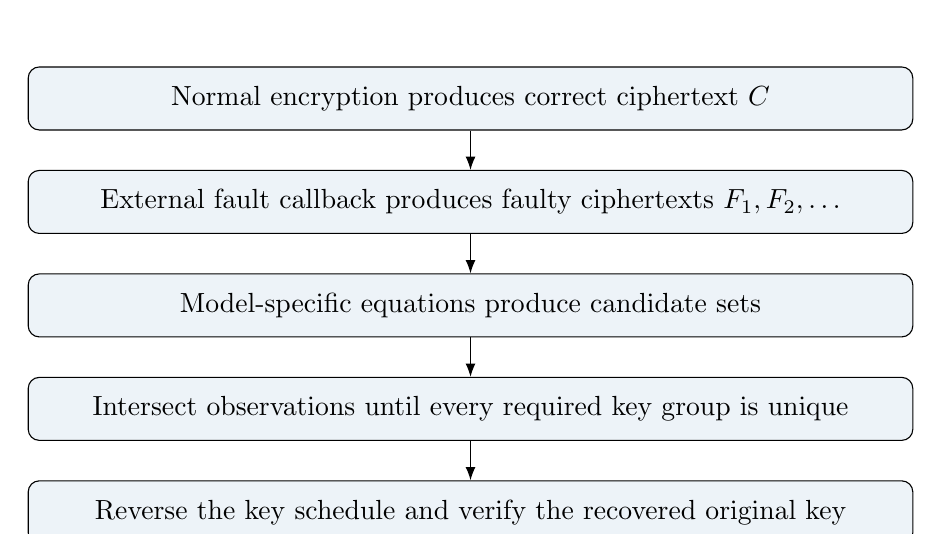
\begin{tikzpicture}[node distance=5mm,box/.style={draw,rounded corners,fill=pale,text width=11cm,align=center,minimum height=8mm},>=Latex]
\node[box] (a) {Normal encryption produces correct ciphertext $C$};
\node[box,below=of a] (b) {External fault callback produces faulty ciphertexts $F_1,F_2,\ldots$};
\node[box,below=of b] (c) {Model-specific equations produce candidate sets};
\node[box,below=of c] (d) {Intersect observations until every required key group is unique};
\node[box,below=of d] (e) {Reverse the key schedule and verify the recovered original key};
\foreach \x/\y in {a/b,b/c,c/d,d/e}{\draw[->] (\x)--(\y);}
\end{tikzpicture}
\end{center}

\section{AES Piret-style attack: code from injection to the master key}
\subsection{Inject into the real AES implementation}
\texttt{encrypt\_with\_trace} in \texttt{piret.py} installs an observer on \texttt{aes.aes\_encrypt}. The callback waits for \texttt{Before MixColumns} in the selected round and performs \texttt{state[row][column] ^= mask}. It then saves immutable byte snapshots. A zero mask gives a clean trace; nonzero masks represent controlled software faults. The solver does not receive this mask.
\begin{lstlisting}[style=pycode,caption={External Piret fault injection into the real AES engine}]
def encrypt_with_trace(plaintext, key, row=0, column=0, mask=0, fault_round=8):
    """Run aes.py itself; this external observer injects and records the fault.

    Round 8 spreads to four key groups. Round 9 reaches one key quartet.
    No second AES implementation is used by the attacker.
    """
    if not (0 <= row < 4 and 0 <= column < 4 and 0 <= mask <= 255 and fault_round in (8, 9)):
        raise ValueError("Fault: row/column 0..3, mask 0..255, round 8 or 9.")
    trace = []

    def observer(number, operation, state):
        if number == fault_round and operation == "Before MixColumns":
            state[row][column] ^= mask
            trace.append((number, "Fault point", aes.state_to_bytes(state)))
        if number > 0 and operation.startswith("After "):
            trace.append((number, operation[6:], aes.state_to_bytes(state)))

    ciphertext = aes.aes_encrypt(plaintext, key, observer=observer)
    return ciphertext, trace
\end{lstlisting}

\subsection{Convert one output pair into four-byte key candidates}
For column $c$, the output indices are $p_r=4((c-r)\bmod4)+r$, $r=0,1,2,3$. Under a guess $k_r$ for a final-key byte,
\[
d_r(k_r)=S^{-1}(C_{p_r}\xor k_r)\xor S^{-1}(F_{p_r}\xor k_r).
\]
The code first groups the 256 byte guesses by their resulting difference. It then enumerates the \emph{shared} unknown error row $q$ and error value $e$, requiring all four equations $d_r(k_r)=M_{r,q}e$ at once. The Cartesian product combines only compatible byte lists; it does not independently choose arbitrary surviving bytes. This preserves the quartet correlation without enumerating all $2^{32}$ quartets first.
\begin{lstlisting}[style=pycode,caption={Piret candidate quartets with one shared row and error}]
def key_candidates(correct, faulty, column):
    """Derive four-byte K10 candidates from ciphertexts only.

    For each guessed byte k, undo final AddRoundKey and SubBytes:
      d = InvSbox[C[p] XOR k] XOR InvSbox[Cfault[p] XOR k].
    All four differences must fit ONE matrix column times ONE unknown error.
    """
    if len(correct) != 16 or len(faulty) != 16:
        raise ValueError("Ciphertexts must each contain exactly 16 bytes.")
    # Each table maps a possible input difference d to compatible byte guesses.
    # Four small lookups avoid brute-force enumeration of all 2^32 quartets.
    tables = []
    for position in output_positions(column):
        table = [[] for _ in range(256)]
        for guess in range(256):
            delta = INV_SBOX[correct[position] ^ guess] ^ INV_SBOX[faulty[position] ^ guess]
            table[delta].append(guess)
        tables.append(table)
    found = set()
    for unknown_row in range(4):
        for unknown_error in range(1, 256):
            # A single shared row/error must satisfy ALL four equations.
            # Independent byte filtering alone would lose this constraint.
            choices = [tables[r][gf_multiply(MIX_MATRIX[r][unknown_row], unknown_error)] for r in range(4)]
            found.update(product(*choices))
    return found
\end{lstlisting}

\subsection{Round 9 versus the supported round-8 variant}
The GUI's \texttt{pdf\_aes\_lesson} and the terminal's \texttt{run.aes\_demo} use round 9. Each observation affects one output quartet. These functions intersect \texttt{key\_candidates} sets separately for all four columns and place the unique tuples back into their original $K_{10}$ byte positions.

The direct \texttt{piret.py} AES command uses round 8. The additional round spreads the original byte disturbance to all four column groups; each final-round group still satisfies a round-9 one-byte-input differential equation with its own effective error. That effective error is not necessarily the original injected mask. \texttt{recover\_last\_key} therefore processes all four groups from each faulty output. Its explicit requirement that all sixteen ciphertext bytes change belongs to this round-8 path; it must not be imposed on round-9 observations.
\begin{lstlisting}[style=pycode,caption={Round-8 AES recovery: intersect all four output groups}]
def recover_last_key(correct, faulty_outputs, observer=None):
    """Attacker API: no master key, plaintext, fault mask or internal states.

    The optional observer is for logging only; it cannot modify candidate sets.
    A None result means ambiguity, never an arbitrary candidate selection.
    """
    if len(correct) != 16:
        raise ValueError("Correct ciphertext must contain 16 bytes.")
    groups, used = [None] * 4, 0
    for used, faulty in enumerate(faulty_outputs, 1):
        if len(faulty) != 16 or any(a == b for a, b in zip(correct, faulty)):
            raise ValueError("Expected 16 changed output bytes for the round-8 byte-fault model.")
        for column in range(4):
            fresh = key_candidates(correct, faulty, column)
            before = None if groups[column] is None else len(groups[column])
            # An intersection can retain/remove candidates, never introduce new ones.
            groups[column] = fresh if groups[column] is None else groups[column] & fresh
            if not groups[column]:
                raise ValueError("Empty candidate intersection: incompatible ciphertexts or fault model.")
            if observer:
                observer(used, column, before, len(fresh), tuple(sorted(groups[column])))
        if all(len(group) == 1 for group in groups):
            # Group tuples are in pre-ShiftRows row order. Restore true K10 order.
            last_key = bytearray(16)
            for column in range(4):
                for position, byte in zip(output_positions(column), next(iter(groups[column]))):
                    last_key[position] = byte
            return bytes(last_key), used
    return None, used
\end{lstlisting}

\subsection{Recover the original AES key}
Once $K_{10}$ is unique, \texttt{reverse\_key\_schedule} initializes $w_{40},\ldots,w_{43}$ and walks downward. It computes each earlier word with XOR and the forward key-schedule transformation. It never reads the original key. The forward S-box is correct here because its input schedule word is already known.
\begin{lstlisting}[style=pycode,caption={Reverse AES-128 expansion to recover the original key}]
def reverse_key_schedule(last_key, observer=None):
    """AES-128 recurrence reversed: w[i-4] = w[i] XOR transform(w[i-1]).

    Descending order guarantees that both right-hand words are already known.
    Reversal still uses the FORWARD S-box: its input word is known, so there
    is no reason to invert SubWord. This function never reads the master key.
    """
    if len(last_key) != 16:
        raise ValueError("K10 must contain 16 bytes.")
    words = [None] * 44
    # K10 occupies the final four schedule words, w40 through w43.
    words[40:] = [list(last_key[index:index+4]) for index in range(0, 16, 4)]
    for index in range(43, 3, -1):
        transformed = words[index - 1][:]
        if index % 4 == 0:
            # Same RotWord/SubWord/Rcon transformation as forward expansion.
            transformed = [SBOX[byte] for byte in transformed[1:] + transformed[:1]]
            transformed[0] ^= aes.RCON[index // 4]
        words[index - 4] = [a ^ b for a, b in zip(words[index], transformed)]
        if observer:
            observer(index, bytes(words[index]), bytes(transformed), bytes(words[index - 4]))
    return bytes(sum(words[:4], []))
\end{lstlisting}

If a group still has more than one candidate, the lesson reports ambiguity instead of guessing a key. Increasing the number of observations can help, but no fixed success count is guaranteed for every target state and fault sequence.

\section{AES Giraud attack: one-bit filtering and complete recovery}
\subsection{External fault before final SubBytes}
\texttt{giraud.aes\_fault\_encrypt} changes one bit in the state immediately before final-round SubBytes. Byte index $b$ maps to \texttt{state[b \% 4][b // 4]}, consistent with AES column-major storage. Unlike the Piret fault, no MixColumns follows this location; one altered S-box input byte reaches one ciphertext byte after ShiftRows.
\begin{lstlisting}[style=pycode,caption={External single-bit fault before final AES SubBytes}]
def aes_fault_encrypt(plaintext, key, byte=0, mask=None):
    """Interfere with the real aes.py execution before final SubBytes.

    Only this attack callback changes the state. Without it AES is unchanged.
    Snapshots are copies for teaching; they are never inputs to the solver.
    """
    if not 0 <= byte < 16:
        raise ValueError("AES input byte must be 0..15.")
    if mask is not None:
        validate_mask(mask)
    trace = {}

    def observer(number, operation, state):
        if number == 10 and operation == "Before SubBytes":
            trace["Before fault"] = aes.state_to_bytes(state)
            if mask is not None:
                state[byte % 4][byte // 4] ^= mask
            trace["Injected bit"] = aes.state_to_bytes(state)
        if number == 10 and operation.startswith("After "):
            name = "Ciphertext" if operation == "After AddRoundKey" else operation[6:]
            trace[name] = aes.state_to_bytes(state)

    ciphertext = aes.aes_encrypt(plaintext, key, observer=observer)
    return ciphertext, trace
\end{lstlisting}

\subsection{Why the filter works}
\texttt{giraud.aes\_candidates}, listed in the implementation chapter, first requires exactly one changed output byte. For each $k\in\{0,\ldots,255\}$, it computes
\[
\delta(k)=S^{-1}(C_j\xor k)\xor S^{-1}(F_j\xor k).
\]
In unknown-bit mode, it keeps $k$ when $\delta(k)\in\{1,2,4,8,16,32,64,128\}$. In known-bit mode, it requires the stronger condition $\delta(k)=e$ for the supplied exact mask. A one-bit difference is required at the \emph{inverse-S-box input comparison}, not necessarily in the observed ciphertext XOR.

\texttt{giraud.masks\_for} generates up to eight distinct single-bit observations per target byte. \texttt{giraud.intersect\_candidates} intersects the resulting sets. The terminal \texttt{main} and GUI \texttt{giraud\_lesson} repeat this for all sixteen input byte positions, use the observed output index after ShiftRows to assemble $K_{10}$, and call \texttt{piret.reverse\_key\_schedule}. Even after all eight masks, an ambiguous byte must remain reported as ambiguous. Knowing the fault location does not imply knowing its exact bit.

\section{SM4 controlled-byte DFA: code and full-key extension}
\subsection{Inject before tau and undo output diffusion}
\texttt{piret.sm4\_fault\_encrypt} attaches an observer to \texttt{sm4.sm4\_encrypt\_block}. At \texttt{Sbox input}, it applies \texttt{mask << (24 - 8*byte)} to the 32-bit value. The shift preserves big-endian byte numbering. Its diagnostic trace may contain subkeys for teaching; the oracle passed to the solver returns only the faulty ciphertext.

At target round $i$,
\[
A_i=X_{i+1}\xor X_{i+2}\xor X_{i+3}\xor rk_i,
\qquad X_{i+4}=X_i\xor L(\tau(A_i)).
\]
When the round is last in the current view, only $X_{i+4}$ changes. Since $L$ is XOR-linear,
\[
\Delta B_i=L^{-1}(X_{i+4}\xor X'_{i+4}).
\]
\texttt{inverse\_rows} constructs the $32\times32$ binary matrix of $L$ and inverts it by Gaussian elimination. \texttt{inverse\_linear} applies the inverse through binary dot products. This is an inverse of the data diffusion map, not the key-schedule map $L'$.
\subsection{Turn S-box input guesses into key-byte guesses}
For the known fault byte $e$, enumerate $a$ satisfying $S(a)\xor S(a\xor e)=\Delta B_{i,b}$. Let $q$ be byte $b$ of $X_{i+1}\xor X_{i+2}\xor X_{i+3}$, available in the other three words of the view. Then a compatible subkey byte is $a\xor q$. The function validates the unchanged words and single-byte support of $\Delta B_i$ before filtering.
\begin{lstlisting}[style=pycode,caption={Known-byte SM4 differential filtering}]
def sm4_byte_candidates(correct, faulty, byte, mask):
    """Attacker API: outputs and the PDF's KNOWN fault byte/value only."""
    if len(correct) != 16 or len(faulty) != 16 or not 0 <= byte < 4 or not 1 <= mask <= 255:
        raise ValueError("Invalid SM4 output or known-fault descriptor.")
    c, f = struct.unpack(">4I", correct), struct.unpack(">4I", faulty)
    if c[1:] != f[1:]:
        raise ValueError("The last-round model requires three output words unchanged.")
    delta_b = inverse_linear(c[0] ^ f[0])
    shift = 24 - 8 * byte
    if not delta_b or delta_b & ~(255 << shift):
        raise ValueError("Difference does not match a single-byte S-box input fault.")
    d = (delta_b >> shift) & 255
    known = ((c[1] ^ c[2] ^ c[3]) >> shift) & 255
    inputs = {a for a in range(256) if sm4.SBOX[a] ^ sm4.SBOX[a ^ mask] == d}
    return {a ^ known for a in inputs}, inputs, delta_b
\end{lstlisting}

\subsection{Recover four subkeys instead of supplying three reference values}
A single last-round experiment recovers at most $rk_{31}$, which is only 32 bits. The implemented \texttt{piret.recover\_sm4\_master\_key} extends the model:
\begin{enumerate}
\item Recover all four bytes of $rk_{31}$ using faults in round 31.
\item Request new faulty outputs from round 30. Undo round 31 on \emph{both} correct and faulty outputs using the recovered $rk_{31}$.
\item Apply the same last-round equations to this restored round-30 view to recover $rk_{30}$.
\item Repeat at round 29, then round 28, undoing only later rounds whose keys have already been recovered.
\item Pass the recovered keys in the order $[rk_{28},rk_{29},rk_{30},rk_{31}]$ to \texttt{reverse\_sm4}.
\end{enumerate}
For a rolling window $(X_{i+1},X_{i+2},X_{i+3},X_{i+4})$ and a known recovered $rk_i$, the previous word is
\[
X_i=X_{i+4}\xor L\bigl(\tau(X_{i+1}\xor X_{i+2}\xor X_{i+3}\xor rk_i)\bigr).
\]
This is the equation implemented by \texttt{peel\_sm4}, already listed in the implementation chapter. The returned view uses reversed word order so that \texttt{sm4\_byte\_candidates} can reuse its output equations. An earlier-round fault may affect several words of the \emph{raw} final ciphertext; the three-unchanged-word condition is checked after the appropriate peeling.

The full recovery function's inputs are a correct output, a callable \texttt{fault\_oracle(round, byte, mask)}, and model configuration. It receives neither plaintext nor a key schedule. The oracle closure knows the simulation key only to run the target. If any byte remains ambiguous, the function returns \texttt{complete=False} and \texttt{master\_key=None}; it never peels an unrecovered round with a reference key.

\texttt{reverse\_sm4} reverses $K_{i+4}=K_i\xor T'(K_{i+1}\xor K_{i+2}\xor K_{i+3}\xor CK_i)$, using $T'=L'\circ\tau$. After obtaining $K_0,\ldots,K_3$, it XORs the fixed $FK_i$ constants to recover the four original master-key words. Four consecutive round keys are required; knowledge of $rk_{31}$ alone is insufficient.

\section{SM4 Giraud-inspired attack: reuse with a different filter}
\texttt{giraud.sm4\_fault\_encrypt} validates that the simulator mask is a single bit, then reuses the actual SM4 target adapter. \texttt{giraud.sm4\_candidates}, listed earlier, computes $L^{-1}(\Delta X)$ and identifies the changed S-box byte. For each candidate input $a$, unknown-bit mode accepts it if
\[
\exists e\in\{1,2,4,8,16,32,64,128\}:\quad S(a)\xor S(a\xor e)=\Delta B_b.
\]
Known-bit mode tests only the specified $e$. The surviving $a$ values are converted to subkey candidates with the same observable-word XOR as the controlled-byte model.

The following wrapper changes only the candidate filter. It keeps the sequential round recovery, intersections, peeling, and key-schedule reversal shared with the byte-DFA engine. In particular, the parameter \texttt{simulator\_mask} is deliberately not forwarded to \texttt{sm4\_candidates} in unknown-bit mode.
\begin{lstlisting}[style=pycode,caption={Giraud-inspired SM4 wrapper with explicit mask knowledge}]
def recover_sm4_master_key(correct, fault_oracle, first_mask=1, maximum=8, known_bit=False, start_byte=0, observer=None):
    """Full SM4 recovery using single-bit filtering in rounds 31, 30, 29, 28."""
    import piret

    def candidate_filter(clean, faulty, simulator_mask):
        # Unknown-bit mode deliberately does not pass the oracle's mask onward.
        return sm4_candidates(clean, faulty, simulator_mask if known_bit else None)

    return piret.recover_sm4_master_key(correct, fault_oracle, masks_for(first_mask, maximum), start_byte, candidate_filter, observer)
\end{lstlisting}

This division explains why two attacks share a full-key recovery engine without being identical: the allowed error sets and the information supplied to the filter differ. Both require controlled faults at each of rounds 31--28 for full recovery in this implementation.

\section{How the GUI maps to the attack code}
Run \texttt{python src/gui.py} from the repository root. Select the algorithm and operation, load a standard example or enter a 16-byte hexadecimal key and block, then build the lesson.
\begin{itemize}
\item \textbf{Encrypt / Decrypt:} \texttt{aes\_trace} or \texttt{sm4\_trace} observes normal transformations. The inverse operation verifies the input block is recovered.
\item \textbf{AES / Fault analysis:} \texttt{pdf\_aes\_lesson} uses the round-9 Piret path, processes all four columns and recovers $K_0$.
\item \textbf{SM4 / Fault analysis:} \texttt{pdf\_sm4\_lesson} calls \texttt{sm4\_master\_lesson} with the known-byte filter.
\item \textbf{Giraud attack:} \texttt{giraud\_lesson} uses the AES byte filter or routes SM4 to \texttt{sm4\_master\_lesson} with the single-bit filter. The exact-bit checkbox selects whether the solver receives the mask.
\end{itemize}
The GUI row/byte and column fields choose the initial demonstration coordinate, not a restriction to recovering only one key byte. The maximum-observation setting is per target group or byte. A lesson snapshot stores the round, operation, explanation, 16-byte displayed state, details and optional correct reference. Normal steps compare with the previous displayed state; fault steps compare with the corresponding correct state. Red nonzero XOR bytes visualize these comparisons. SM4 scalar intermediates $A$, $\tau(A)$ and $L(\tau(A))$ appear in the details; the rolling state does not change until the new word is appended.

\section{Commands and verified default examples}
\begin{lstlisting}[style=terminal]
# GUI: both algorithms and both fault-analysis models
python src/gui.py
# AES round-8 Piret-style terminal lesson
python src/piret.py --algorithm aes
# AES round-9 Piret and controlled-byte SM4 DFA
python src/run.py
# Controlled-byte SM4 full master-key recovery
python src/piret.py --algorithm sm4
# Unknown-bit Giraud models (default)
python src/giraud.py --algorithm aes
python src/giraud.py --algorithm sm4
# Stronger model: exact single-bit mask given to the solver
python src/giraud.py --algorithm aes --known-bit
python src/giraud.py --algorithm sm4 --known-bit
\end{lstlisting}
On 7 November 2026, the following GUI lesson builders were executed directly without opening a window. Coordinates were zero, first mask was \hex{01}, maximum observations was eight, and Giraud used its default unknown-bit mode. The official inputs and keys given earlier were used.
\begin{center}
\small
\begin{tabular}{p{.34\linewidth}rl}
\toprule Lesson & Faulty outputs used & Recovered original key\\\midrule
AES round-9 Piret & 8 & \hex{000102030405060708090A0B0C0D0E0F}\\
AES Giraud, unknown bit & 35 & \hex{000102030405060708090A0B0C0D0E0F}\\
SM4 known-byte DFA & 32 & \hex{0123456789ABCDEFFEDCBA9876543210}\\
SM4 Giraud-inspired, unknown bit & 35 & \hex{0123456789ABCDEFFEDCBA9876543210}\\
\bottomrule
\end{tabular}
\end{center}
All four returned \texttt{verified=True}. These counts describe these particular deterministic examples, not a bound for arbitrary keys, plaintexts, masks or physical targets. Earlier terminal excerpts use the explicitly known-bit model, which explains why their counts can differ.

\section{Validation and limits of the implementation}
The regression suite checks known-answer vectors, inverse operations, fault propagation, candidate intersections, key-schedule reversal and ambiguous cases. \texttt{tests/test\_cipher\_separation.py} checks that the attacks intervene in the real cipher engines. \texttt{tests/test\_sm4\_full\_recovery.py} tests random keys with a precomputed output-only oracle and blocks \texttt{sm4.key\_expansion} while the recovery solver executes. This guards against accidentally obtaining the key from a reference schedule. \texttt{tests/test\_giraud.py} checks known/unknown-bit filtering and recovery for both algorithms.
\begin{lstlisting}[style=terminal]
python -m unittest discover -s tests -v
python tests/test_crypto_lab.py --gui CryptoTests.test_gui
\end{lstlisting}
The simulated observer is more precise than an uncharacterized physical glitch: it selects a round, intermediate value and bit/byte. No runtime trace or known test key is evidence that a ChipWhisperer glitch on STM32F303 satisfies that model. Physical evaluation must establish the observed fault support and location, then report useful-fault rate, ambiguity and key recovery separately. No additional hardware results are claimed by this code walkthrough.

\chapter*{References and Scope}\addcontentsline{toc}{chapter}{References and Scope}
\begin{enumerate}
\item Student-provided handwritten notes, \emph{AES/SM4 notes}, 27 pages, including AES fundamentals, Piret--Quisquater, SM4 fundamentals, and an SM4 DFA example.
\item NIST, \emph{FIPS 197: Advanced Encryption Standard (AES)} (algorithm and official AES test vector).
\item ISO/IEC 18033-3, \emph{Encryption algorithms --- Part 3: Block ciphers} (SM4 specification); SM4 test vector as reproduced in the supplied notes.
\end{enumerate}
\note{The SM4 DFA chapter uses a deliberately strong fault assumption: known XOR magnitude at a specified S-box input. Experimental fault injection must establish whether that assumption is justified. The included Python code demonstrates full recovery with a simulated multi-round fault oracle; no full physical recovery of all four SM4 final round keys is claimed here.}
\end{document}